\newpage
\section{Suggested solutions: Linear Time-invariant Systems}
\begin{enumerate}

\item Claim: $a[n]*b[n]=b[n]*a[n]$.
\begin{proof}
By definition, the convolution of two discrete-time signals is defined as:
\begin{align*}
    a[n]*b[n]&=\sum_{k=-\infty}^{\infty} a[k]b[n-k].
\end{align*}
Change variables by setting $l=n-k$, so that $k=n-l$, then:
\begin{align*}
    a[n]*b[n]&=\sum_{l=-\infty}^{\infty}a[n-l]b[l]=\sum_{l=-\infty}^{\infty}b[l]a[n-l].
\end{align*}
The last sum is the definition of $b[n]*a[n]$, just with the sum index named $l$, hence $a[n]*b[n]=b[n]*a[n]$. 
\end{proof}
The same approach can be used to prove the commutativity of the continuous-time convolution. Again, substitution of variables, but with integrals. Here is the proof:
\begin{proof}
\begin{align*}
    a(t)*b(t) &= \int_{-\infty}^{\infty}a(\tau)b(t-\tau)d\tau, \\
              &= -\int_{\infty}^{-\infty}a(t-u)b(u)du, \\
              &= \int_{-\infty}^{\infty}b(u)a(t-u)du, \\
              &= b(t) * a(t),
\end{align*}
\end{proof}
where $u=t-\tau$, giving $du=-d\tau$. Note that the minus sign is used to swap the limits. 

\item Consider the running average system, defined as:
$$y[n]=\mathcal{T}\{x[n]\}=\frac{1}{L}\sum_{k=0}^{L-1}x[n-k].$$

\begin{enumerate}[a)]
\item Consider two discrete-time signals $x_{1}[n]$ and $x_{2}[n]$ with arbitrary constants $c_{1},c_{2}$, then:
\begin{align*}
    \mathcal{T}\{c_{1}x_{1}[n]+c_{2}x_{2}[n]\}&=\frac{1}{L}\sum_{j=0}^{L-1}[c_{1}x_{1}[n-j]+c_{2}x_{2}[n-j]], \\
    c_{1}\mathcal{T}\{x_{1}[n]\}+c_{2}\mathcal{T}\{x_{2}[n]\}&=c_{1}\frac{1}{L}\sum_{k=0}^{L-1}x_{1}[n-k]+c_{2}\frac{1}{L}\sum_{l=0}^{L-1}x_{1}[n-l],
\end{align*}
which are equal. 

For time-invariance we have:
\begin{align*}
    \mathcal{T}\{\mathcal{D}\{x[n]\}\}&=\mathcal{T}\{x[n-\tau]\}=\frac{1}{L}\sum_{k=0}^{L-1}x[n-\tau-k], \\
    \mathcal{D}\{\mathcal{T}\{x[n]\}\}&=\mathcal{D}\left\{\frac{1}{L}\sum_{k=0}^{L-1}x[n-k]\right\}=\frac{1}{L}\sum_{k=0}^{L-1}x[n-\tau-k],
\end{align*}
both are equal, so the system is time-invariant. 

\item The impulse response can be determined by $h[n]=\mathcal{T}\{\delta[n]\}$, doing this yields:
$$h[n]=\frac{1}{L}\sum_{k=0}^{L-1}\delta[n-k].$$
The impulse response function is then:
$$h[n]=\begin{cases}
    \frac{1}{L}, \quad n=0,\hdots,L-1, \\
    0, \quad \text{otherwise}.
\end{cases}$$

\item The impulse response has $L$ nonzero values, all of them being $1/L$. 

\item Let $x[n]=e^{i\hat{\omega}_{0}n}$, then if we feed this into our system we get:
$$y[n]=\frac{1}{L}\sum_{k=0}^{L-1}e^{i\hat{\omega}_{0}(n-k)}=\frac{1}{L}e^{i\hat{\omega}_{0}n}\sum_{k=0}^{L-1}e^{-i\hat{\omega}_{0}k}=\frac{1}{L}e^{i\hat{\omega}_{0}n}\left(\frac{1-(e^{-i\hat{\omega}_{0}})^{L}}{1-e^{-i\hat{\omega}_{0}}}\right).$$
The output signal is of the form $Ae^{i\phi}e^{i\hat{\omega}_{0}n}$ as $y[n]$ is then:
$$y[n]=\frac{1}{L}\frac{1-e^{-i\hat{\omega}_{0}L}}{1-e^{-i\hat{\omega}_{0}}}e^{i\hat{\omega}_{0}n}=\frac{1}{L}\frac{1-e^{-i\hat{\omega}_{0}L}}{1-e^{-i\hat{\omega}_{0}}}e^{i\hat{\omega}_{0}n}.$$

\item Take $L=4$, then:
$$y[n]=\frac{1}{4}\frac{1-e^{-i\hat{4\omega}_{0}}}{1-e^{-i\hat{\omega}_{0}}}x[n].$$
Next, consider the cases of input frequencies:
\begin{align*}
    \hat{\omega}&=0,\\
    \hat{\omega}&=\pi,\\
    \hat{\omega}&=0.5\pi,
\end{align*}
in these cases the amplitude of the output is:
\begin{align*}
    A&=\lim_{\hat{\omega}\to 0}\frac{1}{4}\frac{1-e^{-4i\hat{\omega}_{0}}}{1-e^{-i\hat{\omega}_{0}}}=\lim_{\hat{\omega}\to 0}\frac{1}{4}\frac{4ie^{-4i\hat{\omega}_{0}}}{ie^{-i\hat{\omega}_{0}}}=1, \\
    A&=\frac{1}{4}\frac{1-e^{-4i\pi}}{1-e^{-i\pi}}=0,\\
    A&=\frac{1}{4}\frac{1-e^{-4i\pi/2}}{1-e^{-i\pi/2}}=0.
\end{align*}

\item The system $y[n]=\mathcal{T}\{x[n]\}$ is an LTI system and can be written as $y[n]=h[n]*x[n]$, where $h[n]$ is the impulse response function as defined above. 
Then the system can be described as:
$$y_{2}[n]=\mathcal{T}\{\mathcal{T}\{x[n]\}\}=\mathcal{T}\{h[n]*x[n]\}=h[n]*(h[n]*x[n])=(h[n]*h[n])*x[n].$$
We've used associativity of convolution in the final step. Then the system can be described as $y_{2}[n]=h_{2}[n]*x[n]$, 
where $h_{2}[n]=h[n]*h[n]$. Hence, $y_{2}[n]$ is an LTI system, as all LTI system are fully determined by convolution with an impulse response. 

\item Have that $h_{2}[n]=\mathcal{T}\{\mathcal{T}\{\delta[n]\}\}=h[n]*h[n]$, so:
$$h_{2}[n]=\sum_{k=-\infty}^{\infty} h[k]h[n-k]=h[0]h[n]+h[1]h[n-1]+h[2]h[n-2]+h[3]h[n-3]+h[4]h[n-4].$$
Terms with $n<0$ are dropped as these will be $0$ due to $h[n]=0$ for $n<0$. Let's evaluate the values of $h_{2}[n]$ with $L=4$:
\begin{align*}
    h_{2}[0]&=h[0]h[0]+h[1]h[-1]+h[2]h[-2]+h[3]h[-3]+h[4]h[-4] = \frac{1}{L^{2}}, \\
    h_{2}[1]&=h[0]h[1]+h[1]h[0]+h[2]h[-1]+h[3]h[-2]+h[4][-3] =\frac{2}{L^{2}}, \\
    h_{2}[2]&=h[0]h[2]+h[1]h[1]+h[2]h[0]+h[3]h[-1]+h[4]h[-2] = \frac{3}{L^{2}}, \\
    h_{2}[3]&=h[0]h[3]+h[1]h[2]+h[2]h[1]+h[3]h[0]+h[4]h[-1] = \frac{4}{L^{2}}, \\
    h_{2}[4]&=h[0]h[4]+h[1]h[3]+h[2]h[2]+h[3]h[1]+h[4]h[0] = \frac{3}{L^{2}}, \\
    h_{2}[5]&=h[0]h[5]+h[1]h[4]+h[2]h[3]+h[3]h[2]+h[4]h[1] = \frac{2}{L^{2}}, \\
    h_{2}[6]&=h[0]h[6]+h[1]h[5]+h[2]h[4]+h[3]h[3]+h[4]h[2] = \frac{1}{L^{2}},
\end{align*}
while the rest are $0$. Thus:
$$h_{2}[n]=\begin{cases}
    \frac{1}{16}, \quad n=0,6,\\
    \frac{2}{16}, \quad n=1,5,\\
    \frac{3}{16}, \quad n=2,4,\\
    \frac{4}{16}, \quad n=3,\\
    0, \quad \text{otherwise}.
\end{cases}$$

To draw the impulse response function, we write a little program to do it. 
The program is shown in Listing \ref{code12_1}. The impulse response is $0$ for all values of $n$ not shown. 
\lstinputlisting[language=Python, caption=Simple convolution,label=code12_1]{ch10/code/ex10_2g.py}
The output of the program is shown in Figure \ref{h2}.

\begin{marginfigure}
    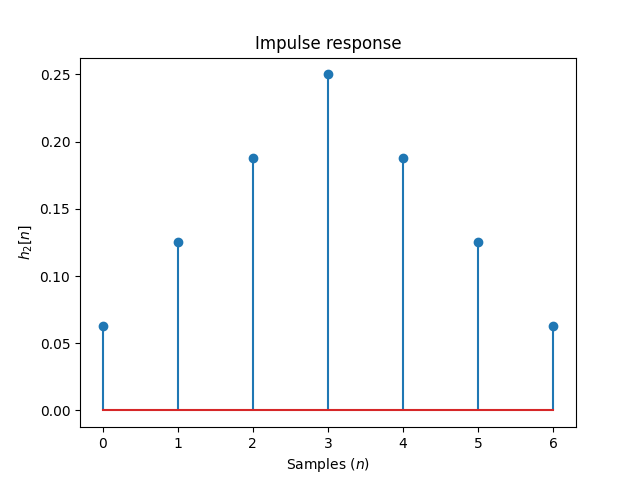
\includegraphics[width=7.5cm,height=6.5cm]{ch10/figures/h2.png}
    \caption{Impulse response for $y_{2}[n]$}
    \label{h2}
\end{marginfigure}
\end{enumerate}

\item Consider the reverb model as shown in Listing \ref{reverb:solution}.
\begin{enumerate}[a)]
    \item By running \verb|reverb.py| and listening to \verb|reverb.wav|, one can 
    hear the reverb effect having been applied to the audio-signal.
    
    \item Running the code yields the figure shown in Figure \ref{reverb:audio}.
    \begin{marginfigure}
    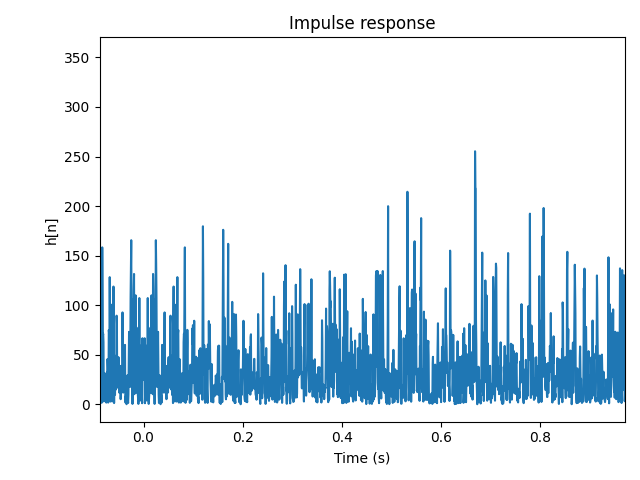
\includegraphics[width=7.5cm,height=7.0cm]{ch10/figures/reverb_impulse.png}
    \caption{Impulse response for the reverb LTI system}
    \label{reverb:audio}
    \end{marginfigure}
    
    \item By changing the \verb|room_length_std| and number of \verb|n_walls| one can get the 
    effect of a small room or a large one. If one increases \verb|room_length_std| the 
    room would be bigger as the echo have to travel further. The impulse response is similar, 
    but the impulse response for a larger room has more peaks at higher times. 
    
    \item To determine $n_{0}$, first consider the time it takes the echo to travel 
    1000 meters and then return. Have that $s=vt$, so $t=s/v$, assuming that 
    the speed is constant throughout. This means that, to travel back and forth takes:
    $$t=\frac{2s}{v}$$
    seconds. The total time in a discrete-time signal is $t=n_{0}T_{s}$, therefore:
    $$n_{0}=\frac{2s}{vT_{s}}=\frac{2sf_{s}}{v},$$
    where $f_{s}$ is the sample length, $s$ is the distance to the surface to scatter 
    from and $v$ is the speed of sound in the corresponding medium. Thus, for an 
    audio-signal sampled at $44100$ Hz, the delay index should be:
    $$n_{0}=\frac{2sf_s}{v}=\frac{(2)(1000\ \text{m})(44100)\ \text{Hz}}{343\ \text{m/s}}\approx257142.85,$$
    or $n_{0}=257143$ to round to the nearest integer. Implementing this with the \verb|reverb.py| 
    script can be accomplished by setting \verb|room_length_std| as 1000, 
    then \verb|n_walls| as 1, \verb|c_sound| as 343 and \verb|sr| as 44100.
    
    \item The average running filter can be implemented by setting the impulse 
    response as $h[n]=\frac{1}{M}\sum_k \delta[n-k]$. The effect on the audio is 
    that the high frequencies are reduced, as expected since the average running filter is a low-pass filter. 

    \lstinputlisting[language=Python,caption=Solution for exercise 3,label=reverb:solution]{ch10/code/ex10_3.py}

\end{enumerate}
\end{enumerate}